%
% quantenfeldtheorie.tex -- Quantenfeldtheorie:  Quantisierung, Schrödinger-Gleichung, der harmonische Oszillator, Photonen als Oszillatoren
%
% (c) 2020 Prof Dr Andreas Müller, Hochschule Rapperswil
%
% !TEX root = ../../buch.tex
% !TEX encoding = UTF-8
%
\section{Quantenfeldtheorie
\label{fourier:section:quantenfeldtheorie}}
\kopfrechts{Quantenfeldtheorie}
Zunächst erfolgt ein Exkurs in die Quantentheorie, um schliesslich zum Laser zu gelangen. % Todo überarbeiten; evtl. weglassen

...
Energie wird in Form von Quanten gespeichert.
Vielfache der Grundfrequenz sind möglich.

Elektromagnetisches Feld $\rightarrow$ Fourier $\rightarrow$ Feldgleichung wie Gleichung vom Federpendel

\subsection{Der harmonische Oszillator
\label{fourier:subsection:derHarmonischeOszillator}}
Warum genau schauen wir uns den harmonischen Oszillator an?
In der Quantenelektrodynamik werden die elektromagnetischen Felder als quantisierte harmonische Oszillatoren modelliert, deren Energie ebenfalls in Vielfachen von $\hbar\cdot\omega$ vorliegt.
Die Zustände des Feldes (Photonenzahlenzustände) werden durch die Schwingungszustände des harmonischen Oszillators beschrieben.

Diese Quantisierung erklärt, warum Licht in Lasern nicht kontinuierlich, sondern in diskreten Paketen (Photonen) emittiert wird. % todo: diesen Satz an anderer passenden Stelle einfügen

Die Wellengleichung lautet bekanntlich
\begin{equation}
    \frac{\partial^2 u}{\partial t^2} = c^2 \left( \frac{\partial^2 u}{\partial x^2} + \frac{\partial^2 u}{\partial y^2} \right).
\end{equation}
Wenn nun der y-Anteil als konstant betrachtet wird, sind alle partiellen Ableitungen nach y gleich Null.
Dies führt zu der vereinfachten Gleichung
\begin{equation}
    \frac{\partial^2 u}{\partial t^2} = c^2 \frac{\partial^2 u}{\partial x^2}.
\end{equation}
Daraus lässt sich die Differentialgleichung
\begin{equation}
    \ddot{a}(t) = -k^2 a(t)
\end{equation}
aufstellen.
$a(t)$ ist hierbei ein Fourier-Koeffizient des elektromagnetischen Wellenfeldes.
Die Lösung dieser Differentialgleichung lautet
\begin{equation}
    u(t,x) = a_k(t) \cos(kx)
\end{equation}

% Besser sin verwenden --> besser e^ikx verwenden; Überlegen, ob wir komplex arbeiten möchten
% In Präsentation mit cos und im Paper mit e^ikx


% Wichtiger Schritt: Der harmonische Oszillator in der Quantenmechanik --> Unterlagen anschauen. 
% Evtl. Termin mit ihm, um Unklarheiten zu klären.

% Gutes Video, welches den harmonischen Oszillator erklärt.
%       https://www.youtube.com/watch?v=5P19hROy9vk
% quantenmechanik: Energie ist auch Quantisiert;
% Oszillator kann nur auf bestimmten Leveln schwingen.
% Energielevel haben dieselben Abstände (quadratischer Brunnen)

% further theory: https://www.youtube.com/watch?v=OdizRUe84bg&list=PL8W2boV7eVfmdWs3CsaGfoITHURXvHOGm

Diese Gleichung ist analog zur Gleichung eines Federpendels.
Es handelt sich hier um ein "Quanten-Federpendel".    
\begin{figure}
\centering
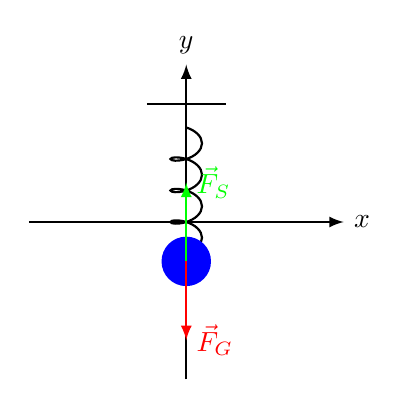
\begin{tikzpicture}[>=latex,thick]
    % Koordinatensystem
    \draw[->] (-2,0) -- (2,0) node[right] {$x$};
    \draw[->] (0,-2) -- (0,2) node[above] {$y$};
    
    % Feder
    \draw[thick] (0,1.5) -- (0,1.2);
    \draw[thick, decorate, decoration={coil, aspect=0.5, segment length=4mm, amplitude=2mm}] (0,1.2) -- (0,-0.5);
    
    % Körper
    \filldraw[blue] (0,-0.5) circle (0.3) node[below] {$m$};
    
    % Kräfte
    \draw[->, thick, red] (0,-0.5) -- (0,-1.5) node[right] {$\vec{F}_G$};
    \draw[->, thick, green] (0,-0.5) -- (0,0.5) node[right] {$\vec{F}_S$};
    
    % Aufhängung
    \draw[thick] (-0.5,1.5) -- (0.5,1.5);
\end{tikzpicture}
\caption{Federpendel}
\label{fourier:figure:federpendel}
\end{figure}